 %% Copyright (C) 2011, Andrea Cimino, All Rights Reserved.
 %% This file is distributed under the terms of the Creative Commons
 %% Licence Non-Commercial Share-Alike license

%% Useful stuff for separate compilation.
\ifx\ismaindoc\undefined
\providecommand{\inbpdocument}{
 \documentclass[11pt,a4paper,twoside,titlepage]{scrbook}
%%%%%%%%%%%%%%%%%%%%%%%%%%%%%%%%
%%%%%%%%%%% PACKAGES %%%%%%%%%%%
%%%%%%%%%%%%%%%%%%%%%%%%%%%%%%%%
% encoding
\usepackage[utf8x]{inputenc}
\usepackage[italian]{babel} % babel (suddivisione parole in sillabe)

\usepackage{amsfonts} % matematica
\usepackage{amsmath} % matematica
\usepackage{amssymb} % simboli vari
\usepackage{calrsfs}
\usepackage{caption}
\usepackage{enumerate}
\usepackage{extarrows} % matematica
\usepackage{keyval}
\usepackage{manfnt} % Simboli curva
\usepackage{mathtools} % matematica
\usepackage{multirow} 
\usepackage[usenames, dvipsnames]{color} % colori con nome
\usepackage[pdftex]{graphicx}
\usepackage{epstopdf} % gestione file EPS
\usepackage{wrapfig} % per figure circondate da testo
\usepackage{framed}	% teoremi framed
\usepackage{fancyhdr} % header buffi
\usepackage[T1]{fontenc} % gestione hbox e vbox
\usepackage[a4paper]{geometry}
\usepackage{microtype} % gestione hbox e vbox
\usepackage[thref, amsthm, amsmath, framed, hyperref]{ntheorem} % teoremi (avanzata)
%% \usepackage{prooftree} % gestione prof-tree
\usepackage{rotating}
\usepackage{stmaryrd}
\usepackage{subfig}
\usepackage{syntax} % syntattic stuff
\usepackage{txfonts}
\usepackage{verbatim} % migliorie al verbatim
%\usepackage{hyperref}
%% \usepackage{qtree}
\usepackage{fancyvrb}
\usepackage{listings}
\usepackage{cancel}
\usepackage{tikz}

\usepackage{bbding} %% Icons

%%%%%%%%%%%%%%%%%%%%%%%%%%%%%%%%
%%%%%%%%%%% GEOMETRY %%%%%%%%%%%
%%%%%%%%%%%%%%%%%%%%%%%%%%%%%%%%
\geometry{verbose,tmargin=2cm,bmargin=2.5cm,lmargin=2.5cm,rmargin=2cm}
\parindent0ex %% Remove paragraph indenting

%%%%%%%%%%%%%%%%%%%%%%%%%%%%%%%%
%%%%%%%%%%% CODE ENV %%%%%%%%%%%
%%%%%%%%%%%%%%%%%%%%%%%%%%%%%%%%
% codice
\newcounter{count}
\setcounter{count}{0}
\newenvironment{code}[1]
{
\color{lightgray}\hrulefill\color{code}
\stepcounter{count} {\bf\small Listato di codice \arabic{count}: {#1} }
\verbatim
}
{
\endverbatim
\color{lightgray}\hrulefill
\color{black}
\\
}

% codice semplice
\newenvironment{simplecode}
{
\color{code} \tt
}
{
\rm
}

 % Notation issues

%% Proof trees.
%\input prooftree
\newcommand*{\nohyp}{\phantom{x}}

%% C++.
\newcommand*{\Cplusplus}{{C\nolinebreak[4]\hspace{-.05em}\raisebox{.4ex}
{\tiny\bf ++}}}

%% BNF rules.
\newcommand*{\vbar}{\mathrel{\mid}}

%% Abstract syntax of the analyzed language.
\newcommand*{\Type}{\mathrm{Type}}
\newcommand*{\dType}{\mathrm{dType}}
\newcommand*{\dT}{\mathrm{dT}}
\newcommand*{\sType}{\mathrm{sType}}
\newcommand*{\sT}{\mathrm{sT}}
\newcommand*{\cType}{\mathrm{cType}}
\newcommand*{\cT}{\mathrm{cT}}
\newcommand*{\Integer}{\mathrm{Integer}}
\newcommand*{\Bool}{\mathrm{Bool}}
\newcommand*{\Id}{\mathrm{Id}}
\newcommand*{\id}{\mathrm{id}}
\newcommand*{\rId}{\mathrm{rId}}
\newcommand*{\idx}{\mathrm{x}}
\newcommand*{\ridx}{\underline{\mathrm{x}}}
\newcommand*{\Exp}{\mathrm{Exp}}
\newcommand*{\Exps}{\mathrm{Exps}}
\newcommand*{\Decl}{\mathrm{Decl}}
\newcommand*{\exceptDecl}{\mathrm{exceptDecl}}
\newcommand*{\Catch}{\mathrm{Catch}}
\newcommand*{\Stmt}{\mathrm{Stmt}}
\newcommand*{\Label}{\mathrm{Label}}
\newcommand*{\Con}{\mathrm{Con}}
\newcommand*{\con}{\mathrm{con}}
\newcommand*{\fps}{\mathrm{fps}}
\newcommand*{\funBody}{\mathrm{Body}}
\newcommand*{\funbody}{\mathrm{body}}
\newcommand*{\main}{\mathrm{main}}
\newcommand*{\es}{\mathrm{es}}
\newcommand*{\formParams}{\mathrm{formParams}}
\newcommand*{\emptysequence}{\boxempty}
\newcommand*{\Glob}{\mathrm{Glob}}

%% Sets of configurations
\newcommand*{\NTe}{\Gamma_\mathrm{e}}
\newcommand*{\NTb}{\Gamma_\mathrm{b}}
\newcommand*{\NTd}{\Gamma_\mathrm{d}}
\newcommand*{\NTg}{\Gamma_\mathrm{g}}
\newcommand*{\NTs}{\Gamma_\mathrm{s}}
\newcommand*{\NTk}{\Gamma_\mathrm{k}}
\newcommand*{\Te}{T_\mathrm{e}}
\newcommand*{\Tb}{T_\mathrm{b}}
\newcommand*{\Td}{T_\mathrm{d}}
\newcommand*{\Tg}{T_\mathrm{g}}
\newcommand*{\Ts}{T_\mathrm{s}}
\newcommand*{\Tk}{T_\mathrm{k}}

%% Lambda notation.
\newcommand*{\lambdaop}{\mathop{\lambda}\nolimits}

%% Sets of (no better specified) configurations.
\newcommand*{\NT}[1]{\Gamma_{#1}}
\newcommand*{\NTq}{\Gamma_q}
\newcommand*{\Tq}{T_q}

%% Denotable values.
\newcommand*{\dVal}{\mathrm{dVal}}
%% Storeable values.
\newcommand*{\sVal}{\mathrm{sVal}}
\newcommand*{\sval}{\mathrm{sval}}

%% Control modes.
\newcommand*{\CtrlMode}{\mathord{\mathrm{CtrlMode}}}
\newcommand*{\cm}{\mathrm{cm}}
%% Branch modes.
%\newcommand*{\BranchMode}{\mathord{\mathrm{BranchMode}}}
\newcommand*{\GotoMode}{\mathord{\mathrm{GotoMode}}}
\newcommand*{\SwitchMode}{\mathord{\mathrm{SwitchMode}}}
\newcommand*{\cmgoto}{\mathop{\mathrm{goto}}\nolimits}
\newcommand*{\cmswitch}{\mathop{\mathrm{switch}}\nolimits}
\newcommand*{\cmbreak}{\mathop{\mathrm{break}}\nolimits}
\newcommand*{\cmcontinue}{\mathop{\mathrm{continue}}\nolimits}
\newcommand*{\cmreturn}{\mathop{\mathrm{return}}\nolimits}
%% Exec mode.
\newcommand*{\cmexec}{\mathrm{exec}}
%% Value mode.
\newcommand*{\ValMode}{\mathord{\mathrm{ValMode}}}
\newcommand*{\cmvalue}{\mathop{\mathrm{value}}\nolimits}
%% Environment mode.
\newcommand*{\EnvMode}{\mathord{\mathrm{EnvMode}}}
\newcommand*{\cmenv}{\mathrm{env}}
%% Exception modes.
\newcommand*{\ExceptMode}{\mathord{\mathrm{ExceptMode}}}
\newcommand*{\cmexcept}{\mathrm{except}}

%% Control states.
\newcommand*{\CtrlState}{\mathord{\mathrm{CtrlState}}}
\newcommand*{\cs}{\mathord{\mathrm{cs}}}
%% Value states.
\newcommand*{\ValState}{\mathord{\mathrm{ValState}}}
\newcommand*{\valstate}{\upsilon}
%% Environment states.
%\newcommand*{\EnvState}{\mathord{\mathrm{EnvState}}}
%% Exception states.
\newcommand*{\ExceptState}{\mathord{\mathrm{ExceptState}}}
\newcommand*{\exceptstate}{\varepsilon}

%% Keywords.
\newcommand*{\kw}[1]{\mathop{\textup{\textbf{#1}}}}

\newcommand*{\bop}{\mathbin{\mathrm{bop}}}
%\newcommand*{\uop}{\mathop{\mathrm{uop}}}

%% Things that hold by definition.
\newcommand{\defrel}[1]{\mathrel{\buildrel \mathrm{def} \over {#1}}}
\newcommand{\defeq}{\defrel{=}}
\newcommand{\defiff}{\defrel{\Longleftrightarrow}}
%\newcommand{\defeq}{=}
%\newcommand{\defiff}{\Longleftrightarrow}

%% Divergence relation
\newcommand{\diverges}{\,\mathord{\buildrel \infty \over \longrightarrow}}

%% Special letters denoting sets and algebras.
\providecommand*{\Nset}{\mathbb{N}}             % Naturals
\providecommand*{\Qset}{\mathbb{Q}}             % Rationals
\providecommand*{\Zset}{\mathbb{Z}}             % Integers
\providecommand*{\Rset}{\mathbb{R}}             % Reals

%% Calligraphic alphabet.
\newcommand*{\calA}{\ensuremath{\mathcal{A}}}
\newcommand*{\calB}{\ensuremath{\mathcal{B}}}
\newcommand*{\calC}{\ensuremath{\mathcal{C}}}
\newcommand*{\calD}{\ensuremath{\mathcal{D}}}
\newcommand*{\calE}{\ensuremath{\mathcal{E}}}
\newcommand*{\calF}{\ensuremath{\mathcal{F}}}
\newcommand*{\calG}{\ensuremath{\mathcal{G}}}
\newcommand*{\calH}{\ensuremath{\mathcal{H}}}
\newcommand*{\calI}{\ensuremath{\mathcal{I}}}
\newcommand*{\calJ}{\ensuremath{\mathcal{J}}}
\newcommand*{\calK}{\ensuremath{\mathcal{K}}}
\newcommand*{\calL}{\ensuremath{\mathcal{L}}}
\newcommand*{\calM}{\ensuremath{\mathcal{M}}}
\newcommand*{\calN}{\ensuremath{\mathcal{N}}}
\newcommand*{\calO}{\ensuremath{\mathcal{O}}}
\newcommand*{\calP}{\ensuremath{\mathcal{P}}}
\newcommand*{\calQ}{\ensuremath{\mathcal{Q}}}
\newcommand*{\calR}{\ensuremath{\mathcal{R}}}
\newcommand*{\calS}{\ensuremath{\mathcal{S}}}
\newcommand*{\calT}{\ensuremath{\mathcal{T}}}
\newcommand*{\calU}{\ensuremath{\mathcal{U}}}
\newcommand*{\calV}{\ensuremath{\mathcal{V}}}
\newcommand*{\calW}{\ensuremath{\mathcal{W}}}
\newcommand*{\calX}{\ensuremath{\mathcal{X}}}
\newcommand*{\calY}{\ensuremath{\mathcal{Y}}}
\newcommand*{\calZ}{\ensuremath{\mathcal{Z}}}

%% Declarators for functions and relations.
\newcommand*{\reld}[3]{\mathord{#1}\subseteq#2\times#3}
\newcommand*{\fund}[3]{\mathord{#1}\colon#2\to#3}
\newcommand*{\pard}[3]{\mathord{#1}\colon#2\rightarrowtail#3}

%% Logical quantifiers stuff.
\newcommand{\st}{\mathrel{.}}
\newcommand{\itc}{\mathrel{:}}

%% Domain, codomain and range of a function.
\newcommand*{\dom}{\mathop{\mathrm{dom}}\nolimits}
%\newcommand*{\cod}{\mathop{\mathrm{cod}}\nolimits}
%\newcommand*{\range}{\mathop{\mathrm{range}}\nolimits}

%% Restriction of a function.
\newcommand*{\restrict}[1]{\mathop{\mid}\nolimits_{#1}}

%% Type of a constant.
\newcommand*{\type}{\mathop{\mathrm{type}}\nolimits}

%% Lubs, glbs, and fixed points.
\newcommand*{\lub}{\mathop{\mathrm{lub}}\nolimits}
%\newcommand*{\glb}{\mathop{\mathrm{glb}}\nolimits}
\newcommand*{\lfp}{\mathop{\mathrm{lfp}}\nolimits}
\newcommand*{\gfp}{\mathop{\mathrm{gfp}}\nolimits}

%% Generic widening.
\newcommand*{\widen}{\mathbin{\nabla}}

%% Set theory.
\renewcommand{\emptyset}{\varnothing}

%\newcommand*{\wpc}{\mathop{\wp_\mathrm{c}}\nolimits}
%\newcommand*{\wpf}{\mathop{\wp_\mathrm{f}}\nolimits}
%\newcommand*{\wpn}{\mathop{\wp_\mathrm{n}}\nolimits}

\newcommand*{\sseq}{\subseteq}
\newcommand*{\sseqf}{\mathrel{\subseteq_\mathrm{f}}}
\newcommand*{\sslt}{\subset}
%\newcommand*{\Sseq}{\supseteq}
%\newcommand*{\Ssgt}{\supset}

%\newcommand{\Nsseq}{\nsubseteq}

\newcommand*{\union}{\cup}
\newcommand*{\bigunion}{\bigcup}
%\newcommand*{\biginters}{\bigcap}
\newcommand*{\inters}{\cap}
\newcommand*{\setdiff}{\setminus}

\newcommand{\sset}[2]{{\renewcommand{\arraystretch}{1.2}
                      \left\{\,#1 \,\left|\,
                               \begin{array}{@{}l@{}}#2\end{array}
                      \right.   \,\right\}}}

%% Base sets.
\newcommand*{\ttv}{\mathrm{tt}}
\newcommand*{\ffv}{\mathrm{ff}}
\newcommand*{\divop}{\mathbin{/}}
\newcommand*{\modop}{\mathbin{\%}}
\newcommand*{\andop}{\mathbin{\textbf{\textup{and}}}}
\newcommand*{\orop}{\mathbin{\textbf{\textup{or}}}}
\newcommand*{\notop}{\mathop{\textbf{\textup{not}}}}

\newcommand*{\FI}{\mathop{\mathrm{FI}}\nolimits}
\newcommand*{\DI}{\mathop{\mathrm{DI}}\nolimits}
\newcommand*{\SL}{\mathop{\mathrm{SL}}\nolimits}
%\newcommand*{\match}{\mathop{\mathrm{match}}\nolimits}

\newcommand*{\Env}{\mathord{\mathrm{Env}}}
\newcommand*{\emptystring}{\mathord{\epsilon}}

%% Exceptions.
\newcommand*{\RTSExcept}{\mathord{\mathrm{RTSExcept}}}
\newcommand*{\rtsexcept}{\chi}
\newcommand*{\Except}{\mathord{\mathrm{Except}}}
\newcommand*{\except}{\xi}
\newcommand*{\none}{\mathtt{none}}
\newcommand*{\divbyzero}{\mathtt{divbyzero}}
\newcommand*{\stkovflw}{\mathtt{stkovflw}}
\newcommand*{\datovflw}{\mathtt{datovflw}}
\newcommand*{\memerror}{\mathtt{memerror}}
%\newcommand*{\inerror}{\mathtt{inerror}}
%\newcommand*{\nullptr}{\mathtt{nullptr}}
%\newcommand*{\outofboundsptr}{\mathtt{outofboundsptr}}

%% Flags for terminal configurations of catch clauses.
\newcommand*{\caught}{\mathtt{caught}}
\newcommand*{\uncaught}{\mathtt{uncaught}}

%% Static semantics.
\newcommand*{\TEnv}{\mathord{\mathrm{TEnv}}}
\newcommand*{\tinteger}{\mathrm{integer}}
\newcommand*{\tboolean}{\mathrm{boolean}}
\newcommand*{\trtsexcept}{\mathrm{rts\_exception}}

%% Memory structures.
\newcommand*{\Loc}{\mathord{\mathrm{Loc}}}
\newcommand*{\Ind}{\mathrm{Ind}}
\newcommand*{\Addr}{\mathrm{Addr}}
\newcommand*{\Map}{\mathrm{Map}}
%\newcommand*{\eMap}{\mathrm{eMap}}
\newcommand*{\Stack}{\mathord{\mathrm{Stack}}}
\newcommand*{\Mem}{\mathord{\mathrm{Mem}}}
\newcommand*{\stknew}{\mathop{\mathrm{new}_\mathrm{s}}\nolimits}
\newcommand*{\datnew}{\mathop{\mathrm{new}_\mathrm{d}}\nolimits}
\newcommand*{\txtnew}{\mathop{\mathrm{new}_\mathrm{t}}\nolimits}
\newcommand*{\heapnew}{\mathop{\mathrm{new}_\mathrm{h}}\nolimits}
\newcommand*{\heapdel}{\mathop{\mathrm{delete}_\mathrm{h}}\nolimits}
\newcommand*{\datcleanup}{\mathop{\mathrm{cleanup}_\mathrm{d}}\nolimits}
\newcommand*{\smark}{\mathop{\mathrm{mark}_\mathrm{s}}\nolimits}
\newcommand*{\sunmark}{\mathop{\mathrm{unmark}_\mathrm{s}}\nolimits}
\newcommand*{\slink}{\mathop{\mathrm{link}_\mathrm{s}}\nolimits}
\newcommand*{\sunlink}{\mathop{\mathrm{unlink}_\mathrm{s}}\nolimits}
\newcommand*{\asmark}{\mathop{\mathrm{mark}_\mathrm{s}^\sharp}\nolimits}
\newcommand*{\asunmark}{\mathop{\mathrm{unmark}_\mathrm{s}^\sharp}\nolimits}
\newcommand*{\aslink}{\mathop{\mathrm{link}_\mathrm{s}^\sharp}\nolimits}
\newcommand*{\asunlink}{\mathop{\mathrm{unlink}_\mathrm{s}^\sharp}\nolimits}
\newcommand*{\aswiden}{\mathop{\mathrm{widen}}\nolimits}
\newcommand*{\sm}{\dag}
\newcommand*{\fm}{\ddag}
\newcommand*{\topmost}{\mathop{\mathrm{tf}}\nolimits}
%% Short forms of \datcleanup, \sunmark, \sunlink for table.
\newcommand*{\datcleanupshort}{\mathop{\mathrm{cu}_\mathrm{d}}\nolimits}
\newcommand*{\sunmarkshort}{\mathop{\mathrm{um}_\mathrm{s}}\nolimits}
\newcommand*{\sunlinkshort}{\mathop{\mathrm{ul}_\mathrm{s}}\nolimits}

\newcommand*{\location}[1]{\mathord{#1 \; \mathrm{loc}}}
%\newcommand*{\saeval}{\mathop{\mathrm{aeval}}\nolimits}
%\newcommand*{\saupd}{\mathop{\mathrm{aupd}}\nolimits}
\newcommand*{\asupported}{\mathop{\mathrm{supported}^\sharp}\nolimits}
\newcommand*{\aeval}{\mathop{\mathrm{eval}^\sharp}\nolimits}
\newcommand*{\ceval}[1]{\mathop{\mathrm{eval}_{#1}}\nolimits}

%% Abstracts.
\newcommand*{\Abstract}{\mathord{\mathrm{Abstract}}}
\newcommand*{\abs}{\mathord{\mathrm{abs}}}

%% Integer part function.
\newcommand{\intp}{\mathop{\mathrm{int}}\nolimits}

%% Concrete functions and operations.
% Aritmethic
%% \newcommand*{\conadd}{\mathbin{\boxplus}}
%% \newcommand*{\consub}{\mathbin{\boxminus}}
%% \newcommand*{\conmul}{\mathbin{\boxdot}}
%% \newcommand*{\condiv}{\mathbin{\boxslash}}
%% \newcommand*{\conmod}{\mathbin{\boxbar}}
% Boolean
%% \newcommand*{\coneq}{\mathbin{\triangleq}}
%% \newcommand*{\conineq}{\mathbin{\trianglelefteq}}
%% \newcommand*{\conneg}{\mathbin{\daleth}}
%% \newcommand*{\conor}{\mathbin{\triangledown}}
%% \newcommand*{\conand}{\mathbin{\vartriangle}}
\newcommand*{\bneg}{\mathop{\neg}\nolimits}

%% Abstract functions and operations.
% Aritmethic
\newcommand*{\absuminus}{\mathop{\ominus}\nolimits}
\newcommand*{\absadd}{\mathbin{\oplus}}
\newcommand*{\abssub}{\mathbin{\ominus}}
\newcommand*{\absmul}{\mathbin{\odot}}
\newcommand*{\absdiv}{\mathbin{\oslash}}
\newcommand*{\absmod}{\mathbin{\obar}}
% Boolean
\newcommand*{\abseq}{\mathrel{\triangleq}}
\newcommand*{\absneq}{\mathrel{\not\triangleq}}
\newcommand*{\absleq}{\mathrel{\trianglelefteq}}
\newcommand*{\abslt}{\mathrel{\vartriangleleft}}
\newcommand*{\absgeq}{\mathrel{\trianglerighteq}}
\newcommand*{\absgt}{\mathrel{\vartriangleright}}
\newcommand*{\absneg}{\mathrel{\circleddash}}
\newcommand*{\absor}{\mathrel{\ovee}}
\newcommand*{\absand}{\mathrel{\owedge}}

%% Summaries for theorem-like environments
\newcommand{\summary}[1]{\textrm{\textbf{\textup{#1}}}}

%% Filter function extracting the relevant and irrelevant parts.
\newcommand*{\sel}{\mathop{\mathrm{sel}}\nolimits}
\newcommand*{\mem}{\mathop{\mathrm{mem}}\nolimits}

%% Modeling definite exceptions.
%\newcommand*{\None}{\mathrm{None}}

%% Strict Cartesian products.
\newcommand*{\stimes}{\otimes}
\newcommand*{\spair}[2]{{#1} \otimes {#2}}
%\newcommand*{\rstimes}{\rtimes}
%\newcommand*{\rspair}[2]{{#1} \rtimes {#2}}
%\newcommand*{\lstimes}{\ltimes}
%\newcommand*{\lspair}[2]{{#1} \ltimes {#2}}

%% Additional syntax for the numeric type extension supplement
\newcommand*{\iT}{\mathrm{iT}}
\newcommand*{\iType}{\mathrm{iType}}
\newcommand*{\tschar}{\mathrm{signed\_char}}
\newcommand*{\tuchar}{\mathrm{unsigned\_char}}
\newcommand*{\flcon}{\mathrm{fl}}
\newcommand*{\Float}{\mathrm{Float}}
\newcommand*{\sccon}{\mathrm{sc}}
\newcommand*{\sChar}{\mathrm{sChar}}
\newcommand*{\uccon}{\mathrm{uc}}
\newcommand*{\uChar}{\mathrm{uChar}}

%% Additional macros for the extension for extra numeric types
%% Floating point types.
\newcommand*{\tfloat}{\mathrm{float}}
%% Numeric types
\newcommand*{\nType}{\mathrm{nType}}
\newcommand*{\nT}{\mathrm{nT}}

%% Additional macros for the extension to pointer and arrays:
%% Elementary types.
\newcommand*{\eType}{\mathrm{eType}}
\newcommand*{\eT}{\mathrm{eT}}
%% Elementary values.
%\newcommand*{\eValue}{\mathrm{eVal}}
%% Array types.
\newcommand*{\aType}{\mathrm{aType}}
\newcommand*{\aT}{\mathrm{aT}}
%% Record types.
\newcommand*{\rType}{\mathrm{rType}}
\newcommand*{\rT}{\mathrm{rT}}
%% Object types.
\newcommand*{\oType}{\mathrm{oType}}
\newcommand*{\oT}{\mathrm{oT}}
%% Function types.
\newcommand*{\fType}{\mathrm{fType}}
\newcommand*{\fT}{\mathrm{fT}}
%% Memory types.
\newcommand*{\mType}{\mathrm{mType}}
\newcommand*{\mT}{\mathrm{mT}}
%% Pointer types.
\newcommand*{\pType}{\mathrm{pType}}
\newcommand*{\pT}{\mathrm{pT}}
%% Offsets.
\newcommand*{\Offset}{\mathrm{Offset}}
\newcommand*{\nooffset}{\boxempty}
\newcommand*{\indexoffset}[1]{\mathopen{\boldsymbol{[}}{#1}\mathclose{\boldsymbol{]}}}
\newcommand*{\fieldoffset}[1]{\mathop{\boldsymbol{.}}{#1}}
%% Lvalues.
\newcommand*{\lValue}{\mathrm{LValue}}
\newcommand*{\lvalue}{\mathrm{lval}}
%% Rvalues.
\newcommand*{\rValue}{\mathrm{RValue}}
\newcommand*{\rvalue}{\mathrm{rval}}
%%
\newcommand*{\pointer}[1]{{#1}\boldsymbol{\ast}}
\newcommand*{\maddress}[1]{\mathop{\&}{#1}}
\newcommand*{\indirection}[1]{\mathop{\boldsymbol{\ast}}{#1}}
%%
\newcommand*{\locnull}{\mathord{l_\mathrm{null}}}
\newcommand*{\ptrmove}{{\mathop{\mathrm{ptrmove}}\nolimits}}
\newcommand*{\ptrdiff}{{\mathop{\mathrm{ptrdiff}}\nolimits}}
\newcommand*{\ptrcmp}{{\mathop{\mathrm{ptrcmp}}\nolimits}}
%%
\newcommand*{\arraysyntax}[3]{\kw{#1} {#2} \kw{of}\,{#3}}
\newcommand*{\arraytype}[2]{\arraysyntax{array}{#1}{#2}}
\newcommand*{\firstof}{{\mathop{\mathrm{firstof}}\nolimits}}
\newcommand*{\arrayindex}{\mathop{\mathrm{index}}\nolimits}
\newcommand*{\locindex}{\mathop{\mathrm{locindex}}\nolimits}
%%
\newcommand*{\recordsyntax}[3]{\kw{#1} {#2} \kw{of}\,{#3}}
\newcommand*{\recordtype}[2]{\recordsyntax{record}{#1}{#2}}
\newcommand*{\field}{\mathop{\mathrm{field}}\nolimits}
\newcommand*{\locfield}{\mathop{\mathrm{locfield}}\nolimits}
%%
\newcommand*{\NTo}{\Gamma_\mathrm{o}}
\newcommand*{\To}{T_\mathrm{o}}
\newcommand*{\NTl}{\Gamma_\mathrm{l}}
\newcommand*{\Tl}{T_\mathrm{l}}
%\newcommand*{\NTr}{\Gamma_\mathrm{r}}
%\newcommand*{\Tr}{T_\mathrm{r}}
%%
\newcommand*{\arraydatnew}{\mathop{\mathrm{newarray}_\mathrm{d}}\nolimits}
\newcommand*{\arraystknew}{\mathop{\mathrm{newarray}_\mathrm{s}}\nolimits}
\newcommand\Cut{\using\sf cut\thickness.08em\justifies}
\newcommand{\maybeeq}{\mathrel{\buildrel \mathrm{?} \over =}}



\makeatletter
\g@addto@macro\@verbatim\footnotesize
\makeatother



%%%%%%%%%%%%%%%%%%%%%%%%%%%%%%%%
%%%%%%%% THEOREMS FORMAT %%%%%%%
%%%%%%%%%%%%%%%%%%%%%%%%%%%%%%%%
% shaded theorems and proofs command
\definecolor{lightgray}{RGB}{230,230,230}
\def\theoremframecommand{\colorbox{lightgray}}

%%% theorems
\theoremstyle{break}
\theoremheaderfont{\normalfont\bfseries}
\theorembodyfont{\itshape}
\theoremsymbol{\ensuremath{\diamondsuit}}
\theoremseparator{\newline}
\newtheorem{theo}{
\includegraphics[scale=0.11]{imgs/book.png}Teorema}[chapter]

%%% propositions
\theoremstyle{break}
\theoremheaderfont{\normalfont\bfseries}
\theorembodyfont{\itshape}
\theoremsymbol{\ensuremath{\diamondsuit}}
\theoremseparator{\newline}
\newshadedtheorem{proposition}{Proposizione}[chapter]

%%% exercises
\theoremstyle{break}
\theoremheaderfont{\normalfont\bfseries}
\theorembodyfont{\itshape}
\theoremsymbol{\ensuremath{\diamondsuit}}
\theoremseparator{\newline}
\newshadedtheorem{exercise}{Esercizio}[chapter]

%%% propositions
\theoremstyle{break}
\theoremheaderfont{\normalfont\bfseries}
\theorembodyfont{\itshape}
\theoremsymbol{\ensuremath{\diamondsuit}}
\theoremseparator{\newline}
\newshadedtheorem{property}{\PencilRightDown $\; $ Propriet\`a}[chapter]

%%% lemmas
\theoremstyle{break}
\theoremheaderfont{\normalfont\bfseries}
\theorembodyfont{\itshape}
\theoremsymbol{\ensuremath{\diamondsuit}}
\theoremseparator{\newline}
\newshadedtheorem{lemma}[theo]{Lemma}

%%% definitions
\theoremstyle{break}
\theoremsymbol{\ensuremath{\clubsuit}}
\theoremseparator{\newline}
\newshadedtheorem{defn}[theo]{Definizione}

%%% examples
\theoremstyle{break}
\theorembodyfont{\itshape}
\theoremsymbol{\ensuremath{\ast}}
\theoremseparator{\newline}
\newshadedtheorem{example}[theo]{Esempio}

%%% observations
\theoremstyle{break}
\theorembodyfont{\itshape}
\theoremsymbol{\ensuremath{\ast}}
\theoremseparator{\newline}
\newshadedtheorem{observation}[theo]{

\includegraphics[scale=0.06]{imgs/lens.png}
Osservazione
}

%%% notations
\newtheorem*{notaz}{Notazione}

%%% proofs
\newenvironment{thproof}
{
\vskip 0.03cm
\begin{small}
\textit{Dimostrazione. }
\color{code}
}
{
\color{black}
\end{small}
$ \square $
\vskip 0.2cm
}

%Notes
\newenvironment{notes}{%
  \def\FrameCommand{\colorbox{yellow}}%
  \MakeFramed {\FrameRestore}
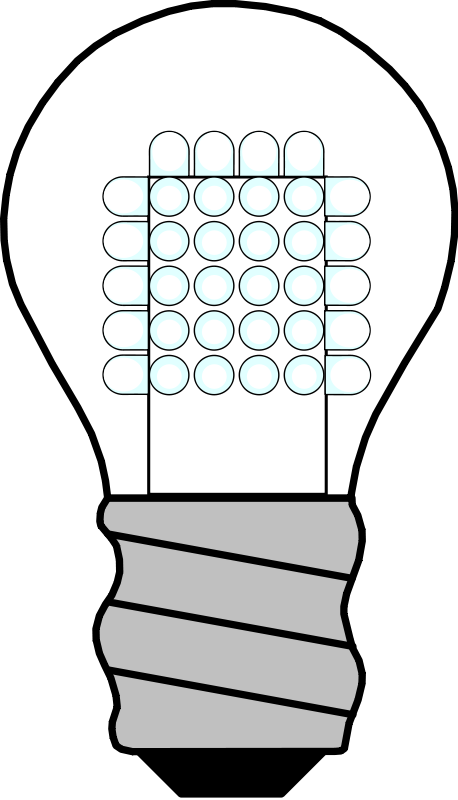
\includegraphics[scale=0.02]{imgs/bulb.png}
 \textbf{Nota} \\
 }%
{\endMakeFramed}

%Work in progress
\newenvironment{workinprogress}{%
  \def\FrameCommand{\colorbox{pink}}%
  \MakeFramed {\FrameRestore}
\lhdbend  \textbf{Work in progress} \\
 }%
{\endMakeFramed}

%Openquestion
\newenvironment{openquestion}{%
  \def\FrameCommand{\colorbox{pink}}%
  \MakeFramed {\FrameRestore}
 \textbf{Domanda aperta} \\
 }%
{\endMakeFramed}

%TODO
\newenvironment{todo}{%
  \def\FrameCommand{\colorbox{pink}}%
  \MakeFramed {\FrameRestore}
 \textbf{TODO} \\
 }%
{\endMakeFramed}

%%%%%%%%%%%%%%%%%%%%%%%%%%%%%%%%
%%%%%%%%%%%% HEADER %%%%%%%%%%%%
%%%%%%%%%%%%%%%%%%%%%%%%%%%%%%%%
\pagestyle{fancy}
% i comandi seguenti impediscono la scrittura in maiuscolo
% dei nomi dei capitoli e dei paragrafi nelle intestazioni
\renewcommand{\chaptermark}[1]{\markboth{#1}{}}
\renewcommand{\sectionmark}[1]{\markright{\thesection\ #1}}
\fancyhf{} % rimuove l'attuale contenuto dell'intestazione
% e del pi\`e di pagina
\fancyhead[LE,RO]{\bfseries\thepage}
\fancyhead[LO]{\bfseries\rightmark}
\fancyhead[RE]{\bfseries\leftmark}
\renewcommand{\headrulewidth}{0.5pt}
\renewcommand{\footrulewidth}{0pt}
\addtolength{\headheight}{0.5pt} % riserva spazio per la linea
\fancypagestyle{plain}{%
\fancyhead{} % ignora, nello stile plain, le intestazioni
\renewcommand{\headrulewidth}{0pt} % e la linea
}


%%%%%%%%%%%%%%%%%%%%%%%%%%%%%%%%
%%%%%%%%%%%% COLORS %%%%%%%%%%%%
%%%%%%%%%%%%%%%%%%%%%%%%%%%%%%%%
\definecolor{code}{gray}{0.3}


%%%%%%%%%%%%%%%%%%%%%%%%%%%%%%%%
%%%%%%%%%%%% NUMBERS %%%%%%%%%%%
%%%%%%%%%%%%%%%%%%%%%%%%%%%%%%%%
\setcounter{tocdepth}{3}
\setcounter{secnumdepth}{3}


%%%%%%%%%%%%%%%%%%%%%%%%%%%%%%%%
%%%%%%%%%%% DOC DATA %%%%%%%%%%%
%%%%%%%%%%%%%%%%%%%%%%%%%%%%%%%%
\title{Appunti di MNO}
\author{Gruppo Informatici Rampanti}
\date{ott 2010 - mag 2011}

\pdfinfo{%
  /Title    (Appunti di MNO)
  /Author   (Andrea Cimino e Lorenzo Muti)
  /Creator  (Andrea Cimino)
  /Producer (Lorenzo Muti)
  /Subject  (MNO)
  /Keywords (MNO)
}


%%%%%%%%%%%%%%%%%%%%%%%%%%%%%%%%
%%%%%%%%%%%%% UTILS %%%%%%%%%%%%
%%%%%%%%%%%%%%%%%%%%%%%%%%%%%%%%
% binary symbols
\newcommand{\modder}{\vdash _{R}}

% vertical gaps
\newcommand{\askip}{\vspace{0.5cm}}
\newcommand{\bskip}{\vspace{1.0cm}}

% various symbols
\newcommand{\qedhere}{\ensuremath{\Box}}
\newcommand{\qed}{\hfill \ensuremath{\Box}}

% substitution
\newcommand{\subst}[2]{^{#1} / _{#2}}

% denotational semantics function names
\newcommand{\bbracket}[1]{\left\llbracket #1 \right\rrbracket}

\newcommand{\aexpr}{\mathcal{A}}
\newcommand{\bexpr}{\mathcal{B}}
\newcommand{\cexpr}{\mathcal{C}}
\newcommand{\Aexpr}[1]{\mathcal{A} \bbracket{#1}}
\newcommand{\Bexpr}[1]{\mathcal{B} \bbracket{#1}}
\newcommand{\Cexpr}[1]{\mathcal{C} \bbracket{#1}}

\newcommand{\semdomset}[1]{(V_{#1})_{\bot}}

% semantic evaluations
\newcommand{\opereval}[3]{\left\langle #1, #2 \right\rangle \rightarrow #3}
\newcommand{\denaeval}[3]{\Aexpr{#1} #2 = #3}
\newcommand{\denbeval}[3]{\Bexpr{#1} #2 = #3}
\newcommand{\denceval}[3]{\Cexpr{#1} #2 = #3}

% rotated sqsubseteqs
\newcommand{\upsqsubseteq}{ $\begin{rotate}{90} $\sqsubseteq$ \end{rotate}$ }
\newcommand{\downsqsubseteq}{ $\begin{rotate}{270} $\sqsubseteq$ \end{rotate}$ }

% Space after paragraph declaration
\makeatletter
\renewcommand\paragraph{\@startsection{paragraph}{4}{\z@}%
  {-3.25ex\@plus -1ex \@minus -.2ex}%
  {1.5ex \@plus .2ex}%
  {\normalfont\normalsize\bfseries}}
\makeatother



% fast theorem and definition
\newcommand{\ftheo}[1]{\colorbox{YellowGreen}{#1}}
\newcommand{\fdefn}[1]{\colorbox{SkyBlue}{#1}}

\theoremstyle{break}
\theoremsymbol{\ensuremath{\clubsuit}}
\theoremseparator{\newline}
\newshadedtheorem{proc}[theo]{Procedura}

% bold math!
\newcommand{\bm}[1]{\mbox{\boldmath{$#1$}}}

\newcommand{\positive}[1]{\textbf{\color{green} +} #1}
\newcommand{\negative}[1]{\textbf{\color{red} -} #1}


\newtheoremlisttype{tab}%
{\begin{tabular*}{\linewidth}{@{}lrl@{\extracolsep{\fill}}r@{}}}%
{##1&##2&##3&##4\\}%
{\end{tabular*}}
\begin{document}
}
\providecommand{\outbpdocument}{\end{document}}
\else
\providecommand{\inbpdocument}{}
\providecommand{\outbpdocument}{}
\fi



\inbpdocument 

% dispensa dft.pdf
%% Bevilacqua 31 Maggio

\chapter{DFT: Trasformata discreta di Fourier}
Non parleremo di interpolazione trigonometrica. \`e un'applicazione
lineare da $\mathbb{C}^{n}$ in $\mathbb{C}^{n}$.  \`e rappresentata
quindi da una matrice, la matrice di Fourier $V \in \mathbb{C}^{n
\times n}$. Questa matrice \`e particolare: può essere
moltiplicata per un vettore $z \in \mathbb{C}^{n}$ in $O(n \log n)$
operazioni aritmetiche.
$$ y = Vz$$
Se invece vogliamo risolvere
$$z = V^{-1}y$$
costa $O(n \log n)$ invece che $O(n^3)$. \\
Un'applicazione \`e la TAC oppure nel calcolo del gradiente coniugato,
dove ad ogni passo di fa un prodotto matrice vettore, il costo passa
da $O(n^2)$ a poco più che lineare.\\ 
Notazione: DFT, IDFT (trasformata inversa). Algoritmo FFT: un algoritmo che
calcola DFT o IDFT.


\begin{defn}[Radice $n$-esima]
Sia $n$ un intero. Si definisce radice $n$-esima dell'unit\`a
ogni numero complesso $z$ tale che $z^{n} = 1$. Una radice n-esima $\omega$ \`e detta
\emph{primitiva} se l'insieme $\{\omega^{i} , i = 0, \ldots , n-1\}$ \`e costituito da 
$n$ elementi distinti. In particolare, indicata con $\mathbf{i}$ l’unit\`a immaginaria ($\mathbf{i}^2 = −1$),
 il numero complesso
$$\omega_n= e^{i 2\pi/n}$$
\`e una radice primitiva $n$-esima dell'unit\`a.
\end{defn}

Una particolare propriet\`a delle radici $n$-esime \`e che possono
essere generate utilizzando una successione di potenze, infatti:
$$
\omega^{k}_{n} = e^{ki 2\pi / n} = \cos k \frac{2\pi}{n} + i \sin k
\frac{2\pi}{n} \qquad k=1, \ldots, n
$$
$V$ \`e la matrice di Vandermonde di ordine $n$, i cui elementi sono
$$ v_{kj} = \omega_{n}^{kj} \qquad k,j = 0, \ldots, n-1 $$


\begin{example}
Per $n = 4$ scegliamo $k=1$ che corrisponde alle serie di potenze
$$ 1 \quad i \quad -1 \quad -i $$

La matrice $V$ contiene tutte le potenze
$$
\begin{pmatrix}
  1 & 1 & 1 & 1 \\
  1 & i & -1 & - i  \\
  1 & -1 & 1 & -1 \\
  1 & -i & -1 & - i
\end{pmatrix}
$$
\end{example}

\begin{property}
$V$ \`e simmetrica (non Hermitiana, perch\`e sui complessi):
 $$V^{T} = V$$
\end{property}

\begin{theo}
 Vale la relazione di ortogonalit\`a:
 \begin{equation}
   \label{dft:01}
    \displaystyle \sum_{j=0}^{n-1} \omega_{n}^{kj} =
      \left\{
      \begin{array}{ll}
        n & \text{ se } k \equiv 0\; (\text{mod } n), \\
        0 & \text{ altrimenti}
      \end{array}
    \right.   
 \end{equation}
 
(Ossia le somme per righe o per colonne sono  $n$ sulla prima riga/colonna,
      0 sulle altre)
\end{theo}
\begin{thproof}
\begin{itemize}
\item Caso  $k \equiv 0  \mod n$:  \\
In questo caso esiste un intero $s$ per cui $k=sn$
e quindi \`e $\omega_{n}^{jk}=1 \quad   \forall j $\\
\begin{comment}
  $$ \displaystyle \sum_{j=1}^{n-1}  \omega_n^{pnj} =
  \displaystyle \sum_{j=0}^{n-1} = n \quad \forall j$$
\end{comment}
\item Caso  $k \not \equiv 0 \mod n$:  \\
  In questo caso \`e $\omega_n^{k} \neq 1$: ponendo
  $x = \omega_n^{k}$ e utilizzando la nota relazione
  (serie geometrica)
  $$(x + x^{2} + \ldots + x^{n-1})(1-x) = 1 - x^{n}$$
  si ottiene
  $$
  \displaystyle (\sum_{j=0}^{n-1} \omega_n^{jk})\underbracket{(1 - \omega_n^{k})}_{\neq 0} 
  = \underbracket{1 - \underbracket{\omega_n^{nk}}_{1}}_{0}
  $$
  e, ricordando che $\omega_n^{k} \neq 1 $ e che $\omega_n^{nk} =1$,
  segue la tesi.
\end{itemize}  
\end{thproof}

\begin{property}
  $$V^{H}V = nI$$
\end{property}
Il risultato si ottiene utilizzando (\ref{dft:01})

\begin{theo}
  $$V^{H}V = nI  \quad \Rightarrow \quad V^{-1} = \dfrac{1}{n}V^{H}$$
\end{theo}
\begin{workinprogress}
  A lezione ha spiegato perch\`e: lascio commentata la dimostrazione
 che va riscritta.
\end{workinprogress}
\begin{comment}
  Inffatti
  $(V^HV)_{rs} = \displaystyle \sum_{k=0}^{n-} \overline{\omega_n}^{kr} \omega_n^{ks}
  = \ldots
  $
  Ma
  Vale inoltre vale la propriet\`a
  $$
  \overline{e^{-i\alpha}} = e^{-i\alpha}
  $$
  quindi
  $\overline{\omega_n}^{kr} = (\overline{e^{kr \dfrac{2\pi}{n}i}}) = \omega_{n}^{-kr}$
  Sostituendo
  $$\ldots \displaystyle \sum \omega_n ^{-kr + ks} =
  \sum_{k=0}^{n-1} \omega_n^{k(s-r)}
  $$
  Abbiamo due casi
  \begin{itemize}
  \item $n$ se $s=r$
  \item $0$ se $s \neq r$
  \end{itemize}
\end{comment}

Una conseguenza \`e che:
$$ z = V^{-1} y \quad \Longleftrightarrow \quad
z = \dfrac{1}{n}V^{H} y$$

\begin{defn}[Trasformata discreta di Fourier]
  L'applicazione
  $$z = \dfrac{1}{n}V^{H} y$$
  \`e detta \emph{trasformata discrata di Fourier} e viene
  generamlmente indicata con la sigla DFT, mentre il vettore
  $z= DFT(y)$ \`e detto \emph{trasformata discreta di Fourier}
  del vettore $y$ e verifica la relazione
  \begin{equation}
    % 74
    \label{fft:02}
    z_j = \dfrac{1}{n} \displaystyle \sum_{k=0}^{n-1}
    y_k \omega_n^{-jk}, \; j=1, \ldots, n-1   
  \end{equation}
\end{defn}

\begin{defn}[Trasformata discreta inversa di Fourier]
  L'applicazione che al vettore $z$ associa il vettore $y$
  \`e detta \emph{trasformata discreta inversa di Fourier}
  e viene generalmente indicata con la sigla IDFT,
  mentre il vettore $y=IDFT(z)$ \`e detto
  \emph{trasformata discreta inversa di Fourier} del vettore
  $z$ e verifica la relazione

\begin{equation}
%75
  \label{fft:03}
  y_k = \displaystyle \sum_{j=0}^{n-1} z_j \omega_n^{jk},
  \;  k =0, \ldots, n-1   
\end{equation}
\end{defn}

Possiamo constatare adesso che possiamo fare il prodotto in $O(n \log n)$ \\
$y = Vz$ prodotto $Vz$: IDFT, trasformata inversa. 
\begin{theo}
  Sia $n = 2^s$ ; il costo computazionale del calcolo della IDFT di un
  vettore $z$ di ordine $n$ o del calcolo della DFT di un vettore $y$ di
  ordine $n$, a meno di termini di ordine inferiore, \`e di $(n/2) \log_2
  n$ moltiplicazioni fra numeri complessi e $n \log_2 $n addizioni fra
  numeri complessi, non contando il calcolo delle $n$ radici $n$-esime
  dell'unit\`a.
\end{theo}

\begin{thproof}
Posto $n=2m$, per la IDFT(z) si ha dalla (\ref{fft:03}):
$$
  \begin{array}{c}
y_k = \displaystyle \sum_{j=0}^{n-1}
z_j \omega_n^{jk} = 
\displaystyle \sum_{j \text{ pari}} z_j \omega_n^{jk}  +
\displaystyle \sum_{j \text{ dispari}} z_j \omega_n^{jk}        
=
\\
\displaystyle \sum_{p=0}^{m-1}z_{2p} \omega_{n}^{2kp}
+
\displaystyle \sum_{p=0}^{m-1}z_{2p+1} \omega_{n}^{k(2p+1)}
  \end{array}
$$
Ponendo $z'_P = z_{2p}$ e $z''_p = z_{2p+1}, p = 0,1, \ldots, m-1$,
si ha
$$
y_k = \displaystyle \sum_{p=0}^{m-1}z'_{p} \omega_{n}^{2kp}
+
\displaystyle \sum_{p=0}^{m-1}z''_{p} \omega_{n}^{k(2p+1)}
$$
Tenendo presente che $\omega_n^{2p} = (\omega_{n/2})^{p} =
\omega_m^{p}$, \`e

\begin{equation}
%81
  \label{fft:04}
y_k = \displaystyle \sum_{p=0}^{m-1}  z'_{p} \omega_{m}^{kp}
+
\omega_n^{k} \displaystyle \sum_{p=0}^{m-1}z''_{p} \omega_{m}^{kp},
\quad k=0, \ldots, n-1  
\end{equation}
Posto $y'=IDFT(z')$ e $y''=IDFT(z'')$, cio\`e
$$
y'_q = \displaystyle \sum_{p=0}^{m-1} z'_p \omega_{m}^{qp},
\quad
y''_q = \displaystyle \sum_{p=0}^{m-1} z_p'' \omega_{m}^{qp},
\quad q=0, \ldots m-1
$$
dalla   (\ref{fft:04}) segue che i primi $m$ elementi
della trasformata sono dati da
\begin{equation}
%82
  \label{fft:05}
y_q = y_q' + \omega_n^{q} y_q^{''}, \quad q=0, \ldots m-1  
\end{equation}
Per calcolare i rimanenti $m$ elementi della trasformata,
poich\'e $\omega^{m} = -1$ e 
$\omega_m^{q+m} = \omega_m^{q}$ dalla
(\ref{fft:04}) segue
$$
y_{q+m} = \displaystyle \sum_{p=0}^{m-1} z'_p \omega_m^{(q+m)p}
 + \omega_n^{q+m} \displaystyle \sum_{p=0}^{m=1} z''_p
\omega_m^{(q+m)p} =
$$
$$
 \displaystyle \sum_{p=0}^{m-1} z'_p \omega_m^{qp}
   + \omega_n^{q+m} \displaystyle 
\sum_{p=0}^{m-1} z''_p \omega_m^{qp} =
$$
\begin{equation}
%83
  \label{fft:06}
y'_q - \omega_n^{q} y_q^{''}, \quad q =0, \ldots m-1  
\end{equation}

La trasformata di ordine $n$ pu\`o quindi essere effettuata
 con 2 trasformate  di ordine $n/2 =m $ pi\`u $n/2= m$ 
moltiplicazioni e $n$ addizioni.
\begin{notes}
  $\omega_m^{qp}$ \`e comune sia per i primi $m$ che per i secondi $m$
elementi, quindi si calcola una volta sola.
Bisogna poi fare 2 volte $m$ somme, quindi $n$ somme in totale.
\end{notes}
 Poich\'e la trasformata di ordine 1 non richiede operazioni, si
possono scrivere le seguenti relazioni di ricorrenza per il numero di
addizioni $A(n)$ e di moltiplicazioni $M (n$) occorrenti per il
calcolo della trasformata di ordine $n$

\begin{equation}
%(84)
  \label{fft:07}
    A(1) = 0, \quad A(n) = 2A(n/2) + n,
\end{equation}
$$ M (1) = 0,\quad  M (n) = 2M (n/2) + n/2.
 $$
Posto $t_s = A(n)$, dove $s=\log_2 n$, dalla (\ref{fft:07}) si
ottiene l'equazione alle differenze
$$t_0 = 0 \quad t_s = 2t_{s-1} + 2^{s} $$
la cui soluzione \`e data da
$$ t_s = s2^s $$
da cui $A(n) = n \log_2 n$. Analogamente si ottiene $M (n) = n/2 log_2
n$. Si procede nello stesso modo per la $DFT(y)$, eseguendo solo al
termine le divisioni per $n$.

\end{thproof}

% Possiamo constatare adesso che possiamo fare il prodotto in $O(n \log n)$ \\
% $y = Vz$ prodotto $Vz$: IDFT, trasformata inversa. \\
% Quand calcoliamo $z = V^{-1}y = \dfrac{1}{n} V^{H} y$: Trasformata diretta DFT.

% Data $y=Vz$ facciamo veere che lo calcoliamo in $O(n \log n)$
% $$ (V)_{kj} = e^{jk \dfrac{2\pi}{n}i} \quad n=2^{s} \quad n=2^{s-1} = \dfrac{n}{2}$$
% $$ y = Vz \quad y_k \displaystyle \sum_{j=0}^{n-1} \omega_n^{kj} z_j =
% \displaystyle \sum_{j \text{ pari}} +
% \displaystyle \sum_{j \text{ dispari}} +
% =
% \ldots =
% \displaystyle \sum_{p=0}^{m-1} \omega_{n}^{2pk} z_{2p} +
%  \omega_{n}^{k}
% \displaystyle \sum_{p=0}^{m-1} \omega_n^{2pk} z_{2p+1}
% = \ldots
% $$
% Il quadrato di $\omega_8$ \`e $\omega_4$, quasto vale in generale
% $$ \omega_n^{2} = \omega_m$$
% $$
% =
% \displaystyle \sum_{p=0}^{m-1} \omega_m^{pk} z_{p+1}
% +
%  \omega_{n}^{k}
% \displaystyle \sum_{p=0}^{m-1} \omega_m^{pk} z_{p+1}
% $$
% $$
% y' = \underbracket{IDFT(z')}_{m} \quad \underbracket{y''= IDFT(z'')}_{m}
% $$
% Le prime $m$ componenti sono possibili con 2 strasformate piccole
% $$q = k = 0, \ldots m=1 $$
% $$\quad y_p = y'_q  + \omega_n^{q} y''_q$$
% Mancano quelle da $m$ a $n-1$
% $$
% \underbracket{y_{m+q}}_{q=0, \ldots, m-1} =
% \displaystyle \sum_{p} \omega_m^{\underbracket{(\cancel{m}+q)}_{k}p}
% z_{2p} + \omega_n^{\underbracket{m+q}_{k}}
% \displaystyle \sum_{p} \omega_{m}^{\underbracket{(\cancel{m}+q)}_{k}p}
% z_{2p+1}
% $$
% $$
% e^{n/2}\dfrac{2\pi}{\pi}i = e^{\pi}
% $$
% Schema ricorsivo
% $$ y_{m+q} = y'_q - \omega_n^{q}y''q$$
\paragraph{Algoritmo}
\begin{enumerate}
\item Si calcolano $\omega_n$ e le sue potenze con espoente
      per $k=0, \ldots, n-1$
\item Calcolo di $y'= IDFT(z')$ di indice pari\\
      Calcolo di $y''= IDFT(z'')$ di indice dispari

\item
$$ y_{m+q} = y'_q - \omega_n^{q}y''q$$
$$\quad y_p = y'_q  + \omega_n^{q} y''_q$$
\end{enumerate}
% Complessit\`a:
% $$M(n) = 2 M(\dfrac{n}{2}) + \dfrac{n}{2} $$
% $$ A(n) = 2A(\dfrac{n}{2}) + n $$
% \\
% \\
% $$M(n) = 2 M(\dfrac{n}{2}) + \dfrac{n}{2}  =
% 2 (2M(\dfrac{n}{4}) + \dfrac{n}{4}) + \dfrac{n}{2} =
% \ldots =
% $$
% Ma $M(1) =0$
% $$
% = \ldots = 2^{s}M(1) + s \dfrac{n}{2}  = \dfrac{n}{2} \log n
% $$
% Per le addizioni
% Viene $A(n) =  n \log n $ \\
Algoritmo FFT pi\`u famoso Cooley-Tuckey e Sande-Tuckey.
Entrambi predisponono l'ordinamento di $v$.
bit reversal.
$$z_0z_1z_2 z_3 z_4 z_5 z_6 z_7$$
$$z_0 z_2 z_4 z_6 \quad z_1 z_3 z_5 z_7 $$
Permutazione di indici.
$$z_0 z_4 z_2 z_6 \quad z_1 z_5  z_3 z_7 $$

\paragraph{Applicazione: Prodotto di polinomi}
$$
2 u(x) = u_0 + u_1x + u_2 x^2  + \underbrace{u_3}_{0} x^{3} + \underbracket{u_4}_{0} x^{4}
2 v(x) =  v_0 + v_1x + v_2 x^2  + \underbrace{v_3}_{0} x^{3} + \underbracket{v_4}_{0} x^{4}
4 z(z)
$$
$$
z(x) = u(x) -v(x) = z_0  + z_1x + z_2 x^{2} + z_3 x^{3} + z_4 x^{4}
$$
$n=5$

$$
\begin{pmatrix}
  u(\omega_5^{0}) \\
  u(\omega_5^{1}) \\
 \ldots
  u(\omega_5^{4}) \\
\end{pmatrix}
=
V
\begin{pmatrix}
  u_1 \\
  u_2 \\
 u_3 \\
 u_4 \\
\end{pmatrix}
\quad
V=
\begin{pmatrix}
 \omega_5^{0} & \omega_5^{1} & \ldots \\
\\
\\
\end{pmatrix}
$$

$$
t = \begin{pmatrix}
  z(\omega_5^0) \\
   \\
  \\
  \\
\end{pmatrix}
\begin{pmatrix}
u(\omega_5^{0} =
  z(\omega_5^0) \\
   \\
  \\
  \\
\end{pmatrix}
$$
\paragraph{Altre applicazioni}
\begin{itemize}
\item Prodotto di interi (\`e come moltiplicare due polinomi)
\item FFT ele matrici circolanti: vengono fuori nei modelli che
     hanno rotazioni (immagine tomografiche)
$$
\begin{pmatrix}
   a_0  & a_1 &  a_2 & a_3 \\
   a_1 & a_2 & a_3 & a_4 \\
   a_2 & a_3 & a_4 & a_1 \\
   a_3 & a_4 & a_1  & a_2 
\end{pmatrix}
$$
Le colonne della matrice di Fourier sono gli autovalori.



\item Im(sfocata) = T Im
Dove T \`e matrice di Toepliz
$$
\begin{pmatrix}
  a & b & c \\
  d & a & b \\
  e & d & a
\end{pmatrix}
$$

$$ t_{ij} = \alpha^{i-j} $$
la Incorniciamo con una 7x7
$$
\begin{pmatrix}
  a & b & c \\
  d & a & b \\
  e & d & a
\end{pmatrix}
$$
Allora diventa circolante.
L'aumento di dimensione \`e compensato dall'uso di DFT.

\end{itemize}
\begin{notes}
All'esame vuole sapere l'idea del costo e di come si fanno i
prodotti.  
\end{notes}

%%% Local Variables: 
%%% mode: latex
%%% TeX-master: "appunti"
%%% End: 

\outbpdocument